\chapter{Distributed Memory MIMD}
A distributed memory MIMD system works on the process level instead of threads (which can be modelled as large grain threads). Messages are passed between processes to facilitate synchronisation and data movement. The important questions are "how to best partition the parallel program?" and "how to best map processes onto the processors to minimise IPC \footnote{Well, it's definitely not instructions-per-clock, but I don't think it's interprocess communication either. Maybe interprocessor communication? As mentioned, acronyms are \textbf{\textit{fun!}}}?"

The design space revolves around reducing the time and frequency of thread switches, which are higher in MIMD machines than in multithreaded architectures. The frequency of computation, as well as the processor time spent on communication, are important factors. The complete design space is depicted in \autoref{fig:screenshot117}.

\begin{figure}
\centering
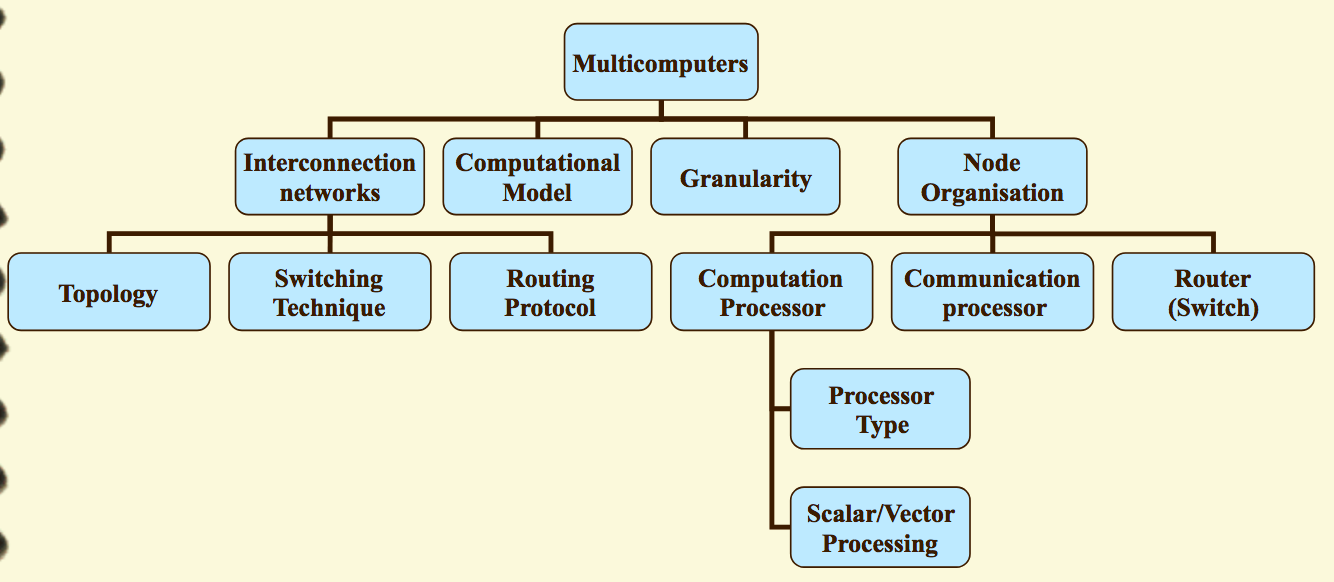
\includegraphics[width=0.7\linewidth]{screenshot117}
\caption{Complete design space for a distributed memory MIMD system.}
\label{fig:screenshot117}
\end{figure}

The design focus is on the organisation of the communication subsystem (especially with regards to the network) and hardware support for message passing. This is often dependent on the algorithms and software in use.

Communication can be conducted over links or channels; the communication graph is mapped onto the underlying network. Nodes consist of a computational processor + private memory, a communication processor, and a router/switch unit.

A multiprocessor can be classified with regards to the following criteria: \begin{itemize}
\item How the interconnection network is organised. \begin{itemize}
	\item Topology \begin{itemize}
		\item Switching technique 
		\item Routing Protocols 
	\end{itemize}
\end{itemize}
\item How the three components of the nodes are composed and integrated: \begin{itemize}
	\item First generation: No communications processor (\autoref{fig:screenshot118}).
	\item Second generation: Separate comms switching units (\autoref{fig:screenshot119}, \autoref{fig:screenshot120}).
	\item Third generation: Separate processors (\autoref{fig:screenshot121}).
\end{itemize}
\item The message passing computational model supported by the multicomputer: \begin{itemize}
	\item Library calls (MPI, PVM, etc) 
	\item CSP support 
	\item Push, pull or active messages 
\end{itemize}
\item The optimal grain of computation: \begin{itemize}
	\item Coarse-grained: Traditional languages.
	\item Medium-grained: CSP.
	\item Fine-grained: Dataflow. 
\end{itemize}
\end{itemize}

\begin{figure}
\centering
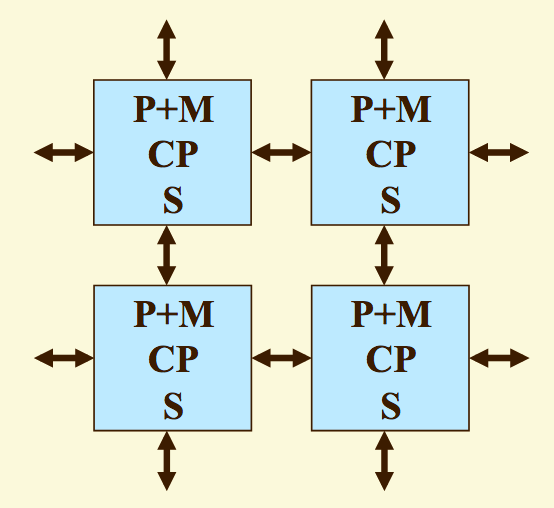
\includegraphics[width=0.5\linewidth]{screenshot118}
\caption{Node organisation: first generation.}
\label{fig:screenshot118}
\end{figure}

\begin{figure}
\centering
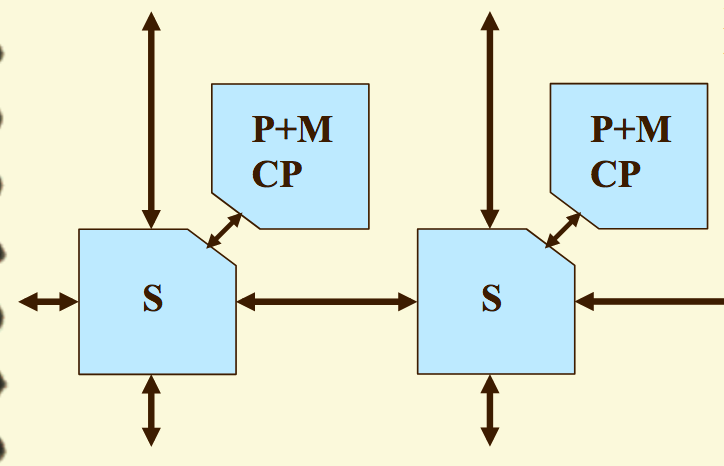
\includegraphics[width=0.5\linewidth]{screenshot119}
\caption{Node organisation: second generation variant 1.}
\label{fig:screenshot119}
\end{figure}

\begin{figure}
\centering
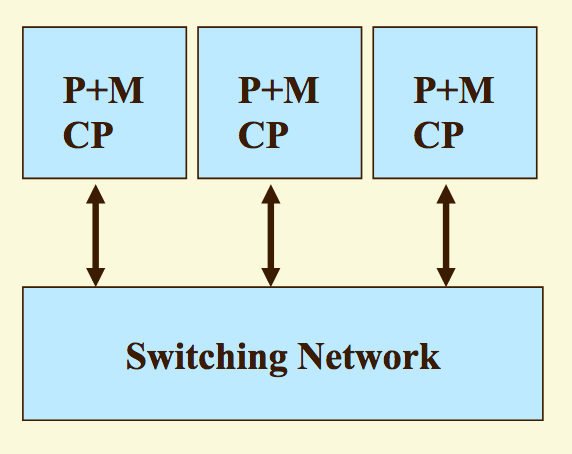
\includegraphics[width=0.5\linewidth]{screenshot120}
\caption{Node organisation: second generation variant 2.}
\label{fig:screenshot120}
\end{figure}

\begin{figure}
\centering
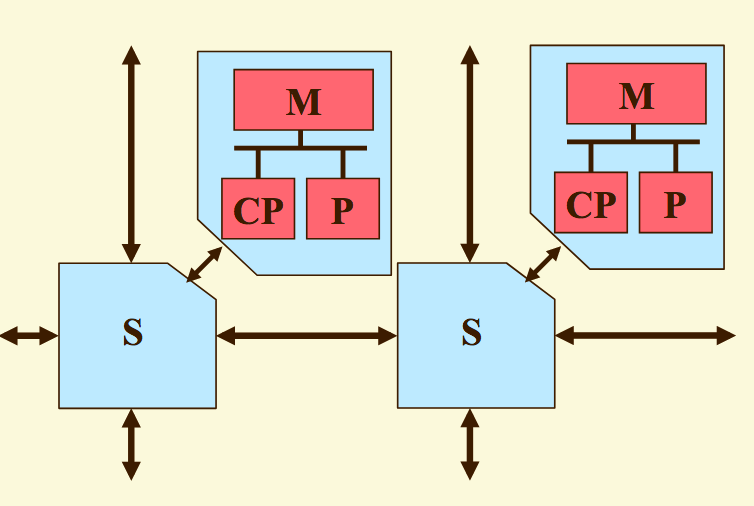
\includegraphics[width=0.5\linewidth]{screenshot121}
\caption{Node organisation: third generation.}
\label{fig:screenshot121}
\end{figure}

\section{Interconnection Network}
The design of the interconnection network is critical to the performance of MIMD machines. Bandwidth and latency are both critical parameters. These networks are characterised by the following: \begin{itemize}
\item \textbf{Network Size (N}): Number of nodes in the network.
\item \textbf{Node Degree (d)}: Number of IO links per node.
\item \textbf{Network diameter (D)}: Maximum number of hops to get from any node to any other.
\item \textbf{Bisection Width (B)}: The minimum number of links broken to break network in 2 equal halves; related to wiring density and overall bandwidth.
\item \textbf{Arc connectivity}: Minimum number of arcs removed to break into two disconnected networks; it is a measure of fault tolerance and contention.
\item \textbf{Cost}: Number of communication links in the network.
\end{itemize}

\begin{figure}
\centering
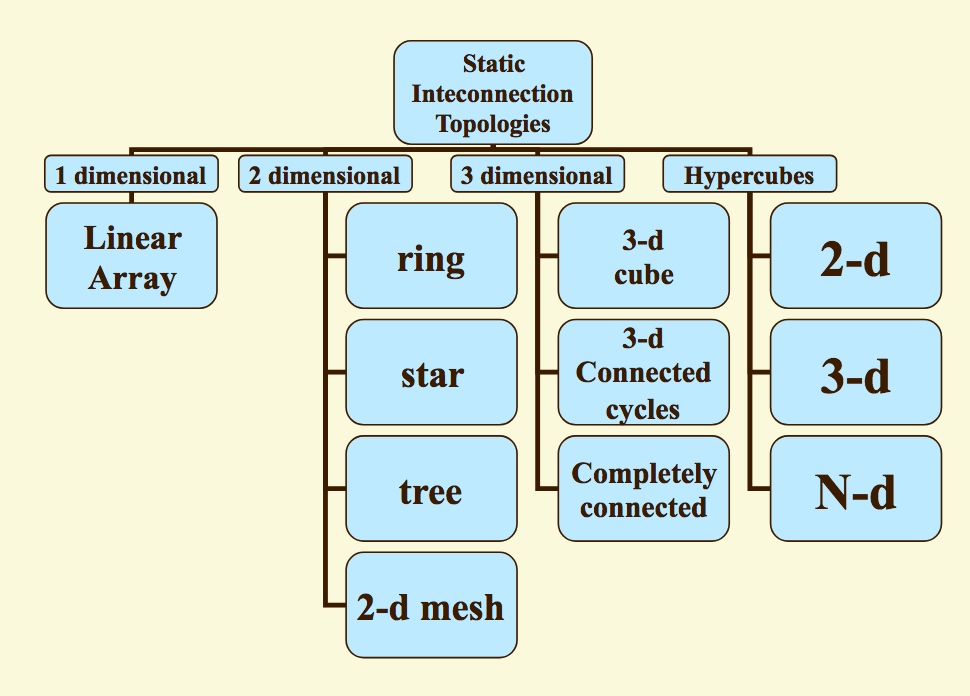
\includegraphics[width=0.7\linewidth]{screenshot122}
\caption{Interconnection topologies.}
\label{fig:screenshot122}
\end{figure}

The possible topologies are shown in a hierarchy in \autoref{fig:screenshot122}. Examples of these are shown in \autoref{fig:screenshot123}, \autoref{fig:screenshot124}, and \autoref{fig:screenshot125}.

\begin{figure}
\centering
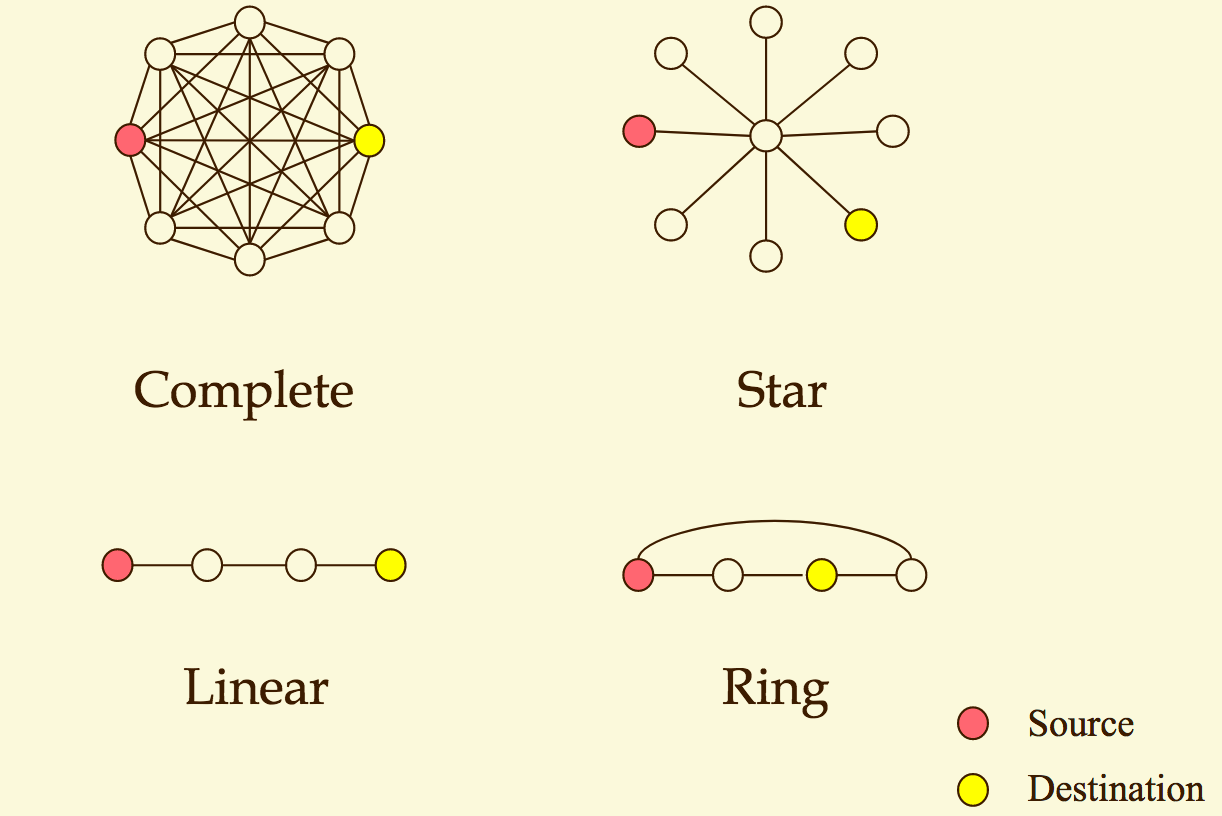
\includegraphics[width=0.7\linewidth]{screenshot123}
\caption{Complete, Star, Linear and Ring network arrangements.}
\label{fig:screenshot123}
\end{figure}

\begin{figure}
\centering
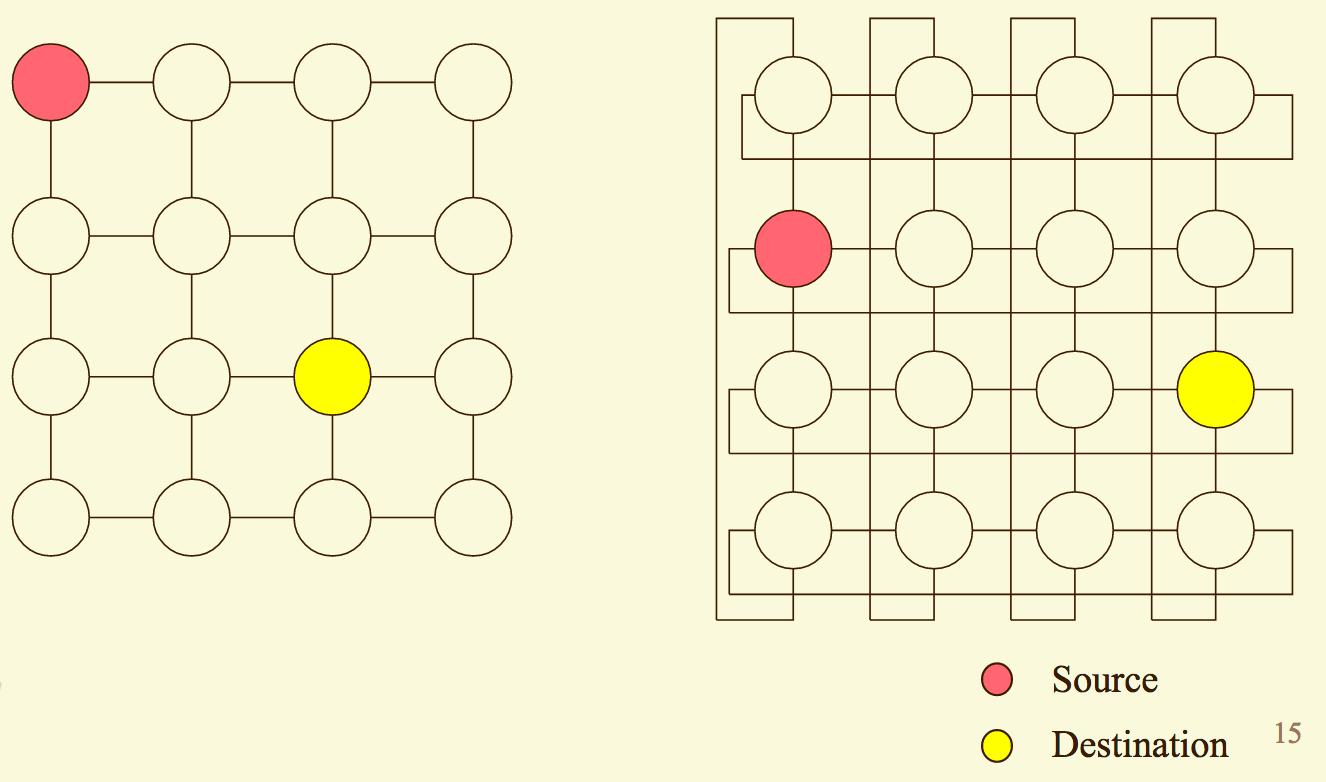
\includegraphics[width=0.7\linewidth]{screenshot124}
\caption{Mesh and Torus network arrangements.}
\label{fig:screenshot124}
\end{figure}

\begin{figure}
\centering
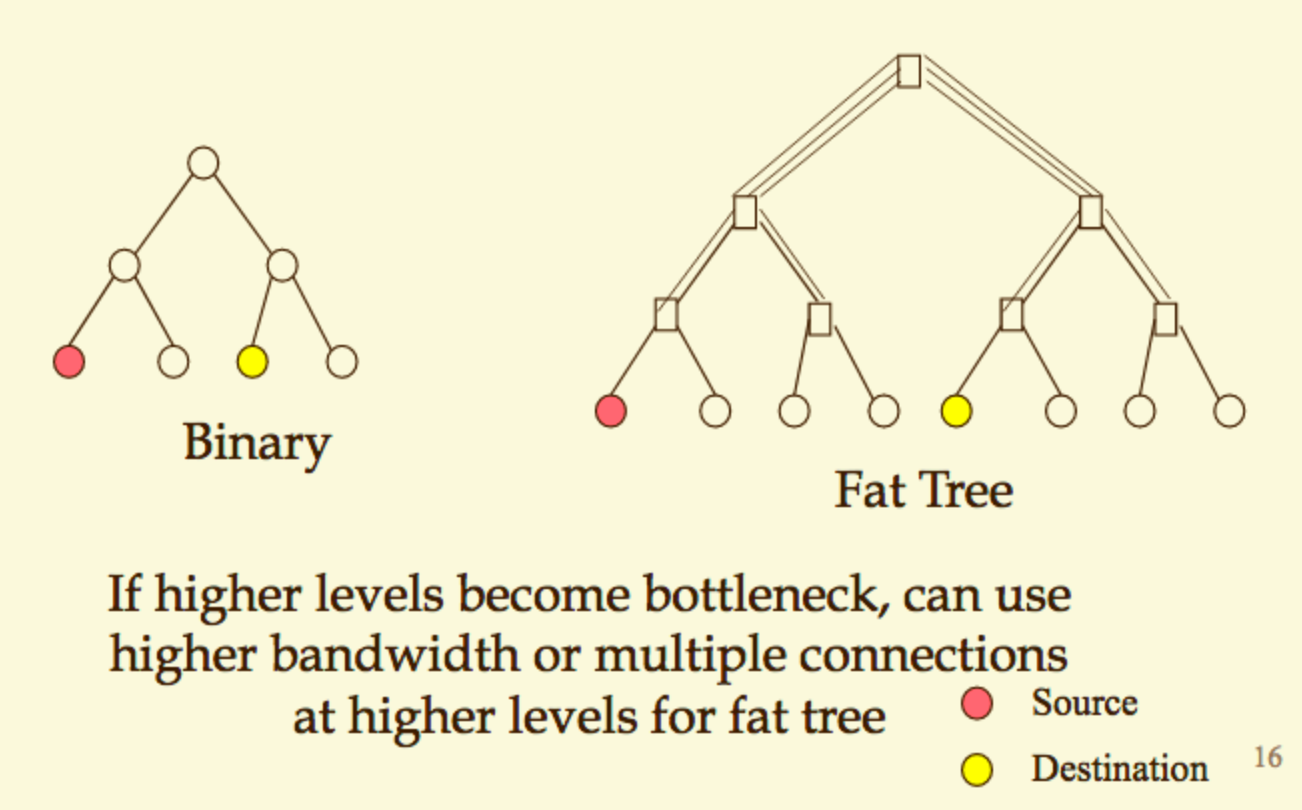
\includegraphics[width=0.7\linewidth]{screenshot125}
\caption{Tree arrangements.}
\label{fig:screenshot125}
\end{figure}

\pagebreak

\begin{figure}
\centering
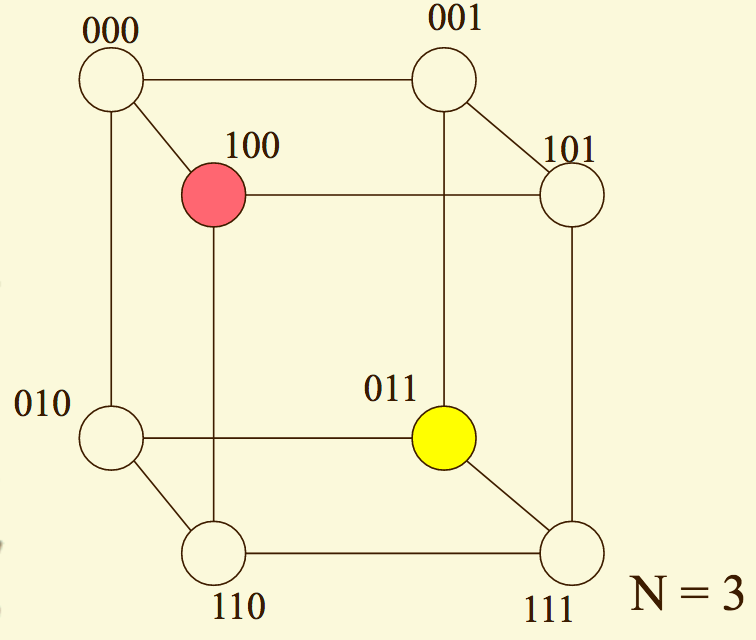
\includegraphics[width=0.7\linewidth]{screenshot126}
\caption{HyperCube network arrangement.}
\label{fig:screenshot126}
\end{figure}

The HyperCube arrangement arranges $2^N$ elements such that each element has $N$ connections to other elements (see \autoref{fig:screenshot126}). Each element is connected to its \textit{boolean} neighbour - that is, the node number differs by only one bit. While it is hard to build scalable fabric with this arrangement, it features good nearest neighbour connectivity, and any element in the arrangement is at most $N$ hops away from another element.

The MultiStage arrangement is a hybrid of the \textit{cross-bar} arrangement and \textit{buses}. They can provide contention-free access (given that multiple requests are not made to the same module) in the general case, but it is worth noting that contention can still occur at certain traffic levels. Unlike buses, they are scalable and can be expanded to accommodate larger systems. As MultiStage is a combination of two arrangements, there are many possible topologies; the simplest is the shuffle exchange network, shown in \autoref{fig:screenshot127}.

\begin{figure}
\centering
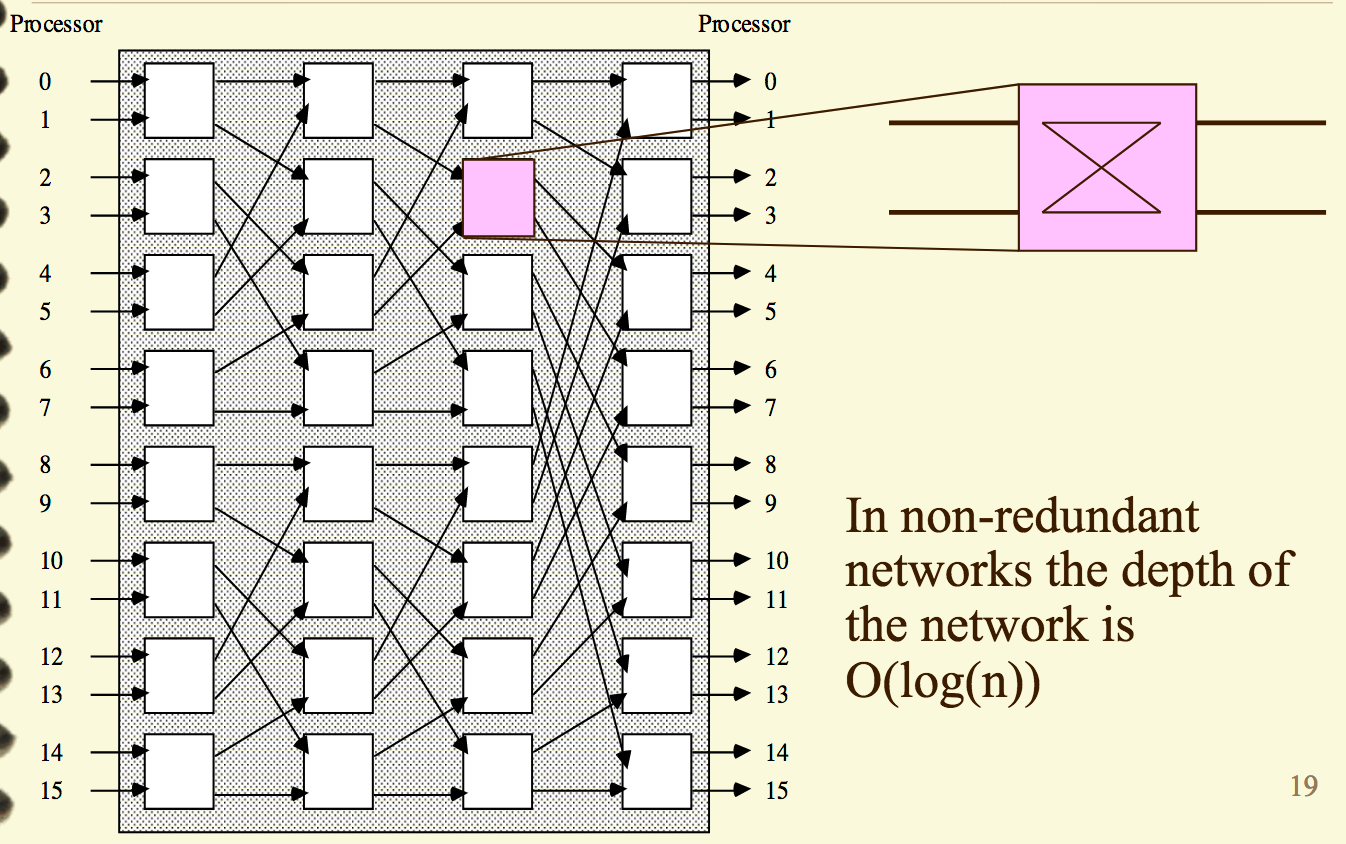
\includegraphics[width=0.7\linewidth]{screenshot127}
\caption{MultiStage network arrangement (shuffle exchange).}
\label{fig:screenshot127}
\end{figure}

Various static network arrangements are compared in \autoref{tab:staticnetworkparameters}.
\begin{table}
\caption{Static network arrangements comparison.}
\label{tab:staticnetworkparameters}
\begin{tabular}{|c|c|c|c|c|c|}
\hline 
\thead{Topology} & \thead{Node \\ degree} & \thead{Diameter} & \thead{Bisection \\ width} & \thead{Arc \\ connectivity} & \thead{Cost} \\ 
\hline 
Linear array & $1$ or $2$ & $N - 1$ & $1$ & $1$ & $N - 1$ \\ 
\hline 
Ring & $2$ & $N/2$ & $2$ & $2$ & $N$ \\ 
\hline 
Star & $1$ or $N-1$ & $2$ & $1$ & $1$ & $N - 1$ \\ 
\hline 
Binary tree & $1$, $2$, or $3$ & $2\log((N+1)/2))$ & $1$ & $1$ & $N - 1$ \\ 
\hline 
2-D mesh & $2$, $3$, or $4$ & $2(N^{1/2}-1)$ & $N^{1/2}$ & $4$ & $2(N-N^{1/2})$ \\ 
\hline 
2-D wraparound & $4$ & $N^{1/2}$ & $2N^{1/2}$ & $4$ & $2N$ \\ 
\hline 
3-D cube & $3$, $4$, $5$, or $6$ & $3(N^{1/3} - 1)$ & $N^{2/3}$ & $3$ & $2(N-N^{2/3})$ \\ 
\hline 
Hypercube & $\log(N)$ & $\log(N)$ & $N/2$ & $\log(N)$ & $(N\log(N))/2$ \\ 
\hline 
Completely connected & $N-1$ & $1$ & $N^2/4$ & $N-1$ & $N(N-1)/2$ \\ 
\hline 
\end{tabular} 
\end{table}

\section{Switching Techniques}
The network structure defines pathways for the data, but switching techniques are responsible for defining how to move data through the network - that is, removing the message from the input buffer and placing it in the output buffer.

\subsection{Packet switching}
Data is divided into packets, which are small packages of data. They include a header, body and tail. The entirety of each packet is stored at each node before being sent on, shown in \autoref{fig:screenshot128}. This means the latency can be described by
\[ \text{Latency} = (\text{Packet length} \times \text{Distance})/\text{Channel Bandwidth} \]
and is shown in graph form in \autoref{fig:screenshot131}.

\begin{figure}
\centering
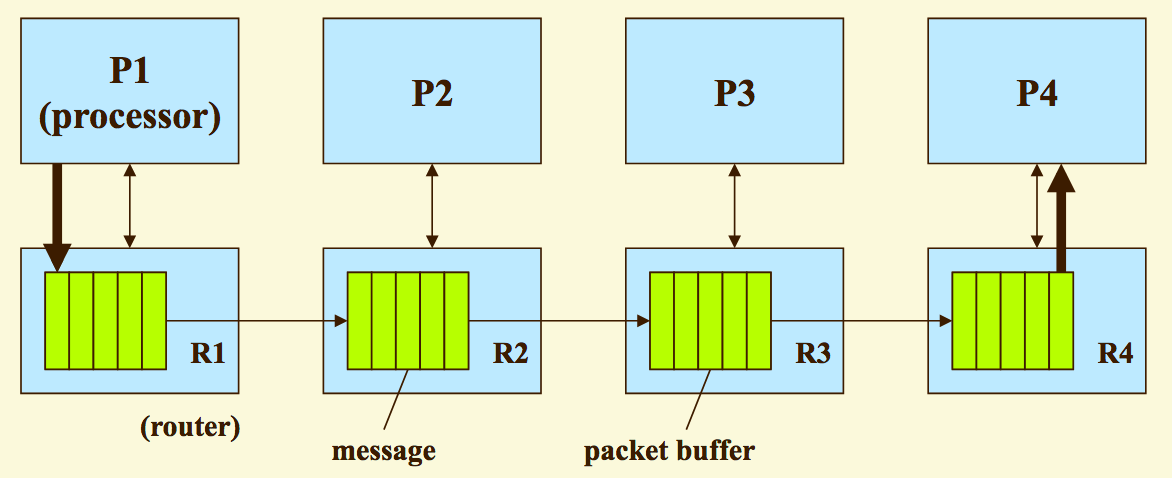
\includegraphics[width=0.7\linewidth]{screenshot128}
\caption{Packet switching.}
\label{fig:screenshot128}
\end{figure}

\begin{figure}
\centering
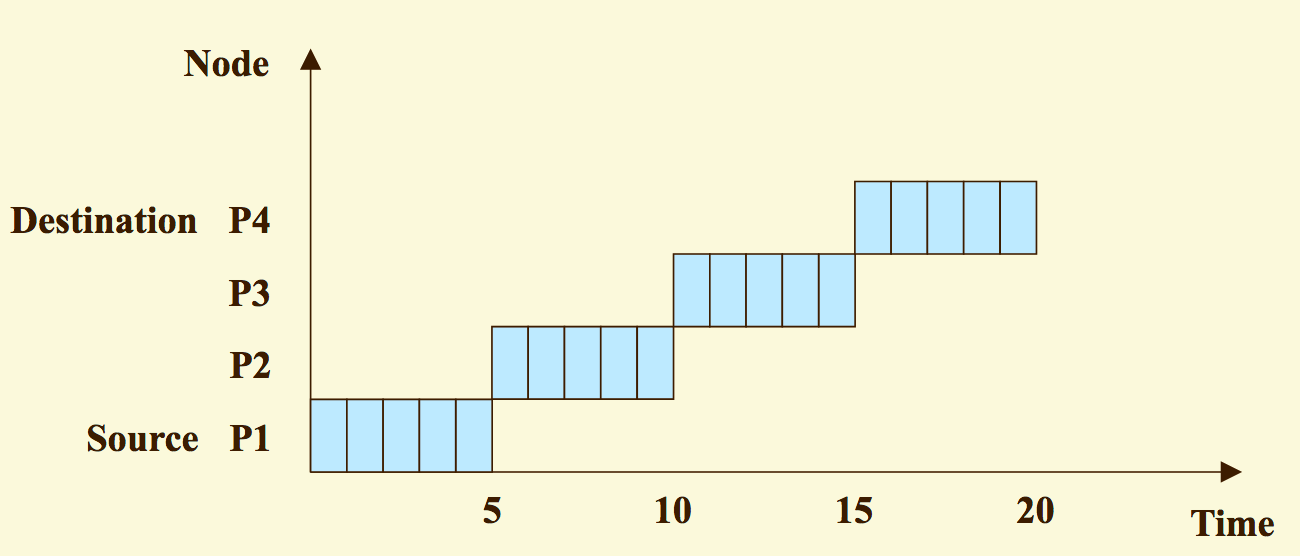
\includegraphics[width=0.7\linewidth]{screenshot131}
\caption{Network latency in packet switching.}
\label{fig:screenshot131}
\end{figure}

\subsection{Circuit switching}
A path between the source and destination is constructed through three distinct phases: \begin{enumerate}
\item \textbf{Circuit establishment phase}: A probe is sent through the network, opening up the path.
\item \textbf{Transmission phase}: The data is sent through the routing path, assuming that it has already been established.
\item \textbf{Termination phase}: The circuit that was constructed is then ripped up.
\end{enumerate}

The latency can be described by
\[ \text{Latency} =  (\text{Probe Length} \times \text{Distance} + \text{Message Length})/\text{Channel Bandwidth} \]
and is shown in graph form in \autoref{fig:screenshot132}.

\begin{figure}
\centering
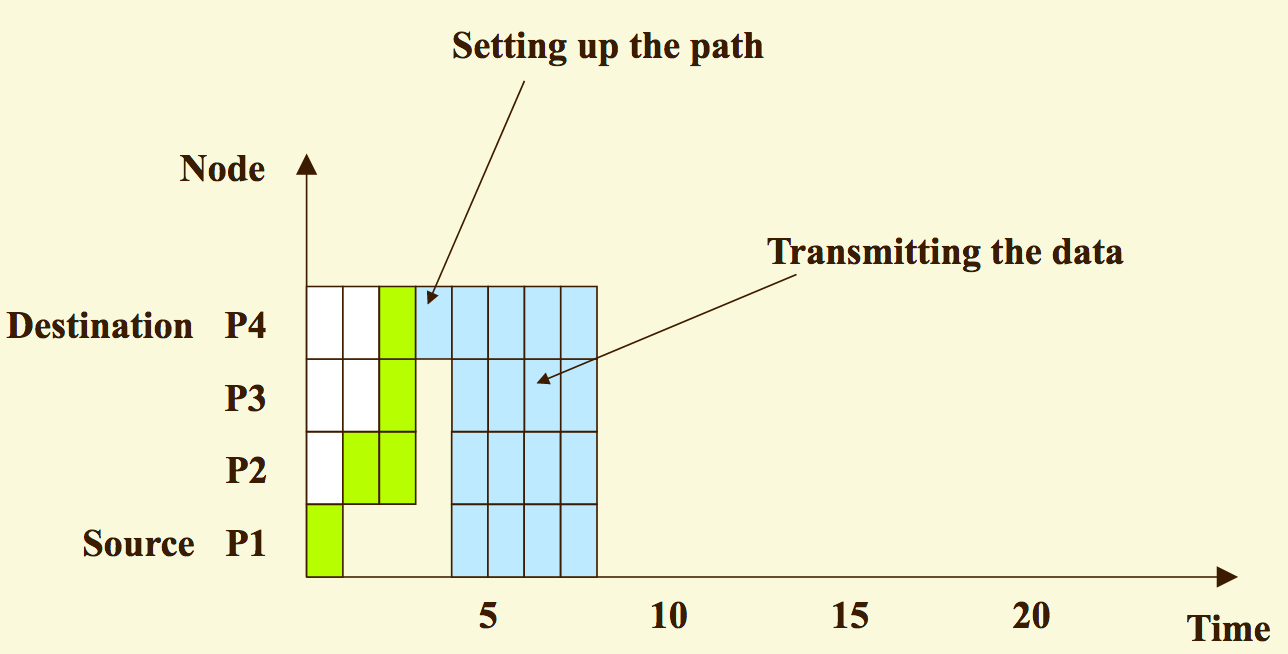
\includegraphics[width=0.7\linewidth]{screenshot132}
\caption{Network latency in circuit switching.}
\label{fig:screenshot132}
\end{figure}


The advantages of circuit switching include not needing to build packets, avoiding the use of buffering, and only having to route once per message (instead of per packet).

\subsection{Virtual cut-through}
Virtual cut-through is a combination of packet switching and circuit switching, shown in \autoref{fig:screenshot129}. The packets are broken into Flow Control Digits (FLITS). If channels are free, FLITS are forwarded in circuit switched mode; otherwise, the message is broken and buffered.

The latency can be described by
\[ \text{Latency} =  (\text{Length of header FLIT} \times \text{Distance} + \text{Message Length})/\text{Channel Bandwidth} \]
and is shown in graph form in \autoref{fig:screenshot133}.

\begin{figure}
\centering
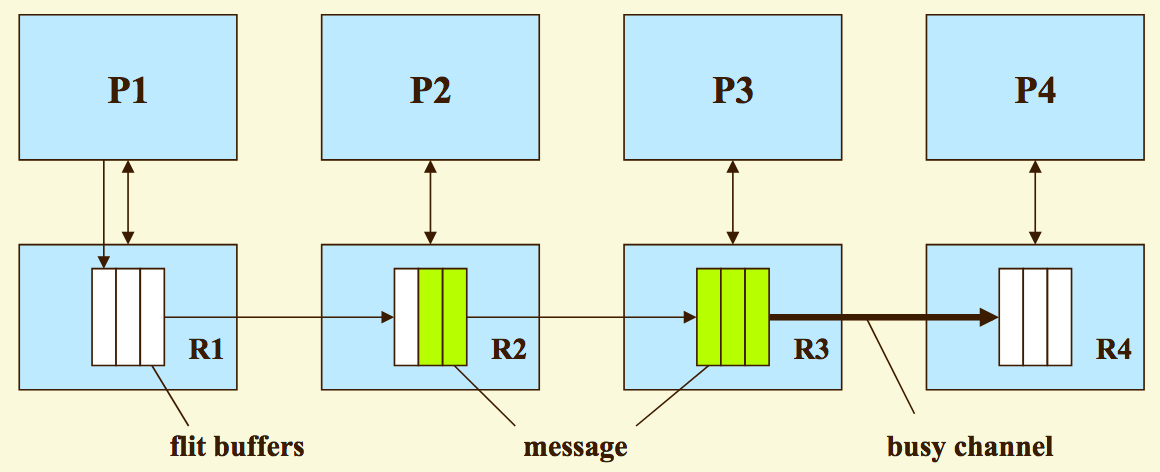
\includegraphics[width=0.7\linewidth]{screenshot129}
\caption{Virtual cut-through.}
\label{fig:screenshot129}
\end{figure}

\begin{figure}
\centering
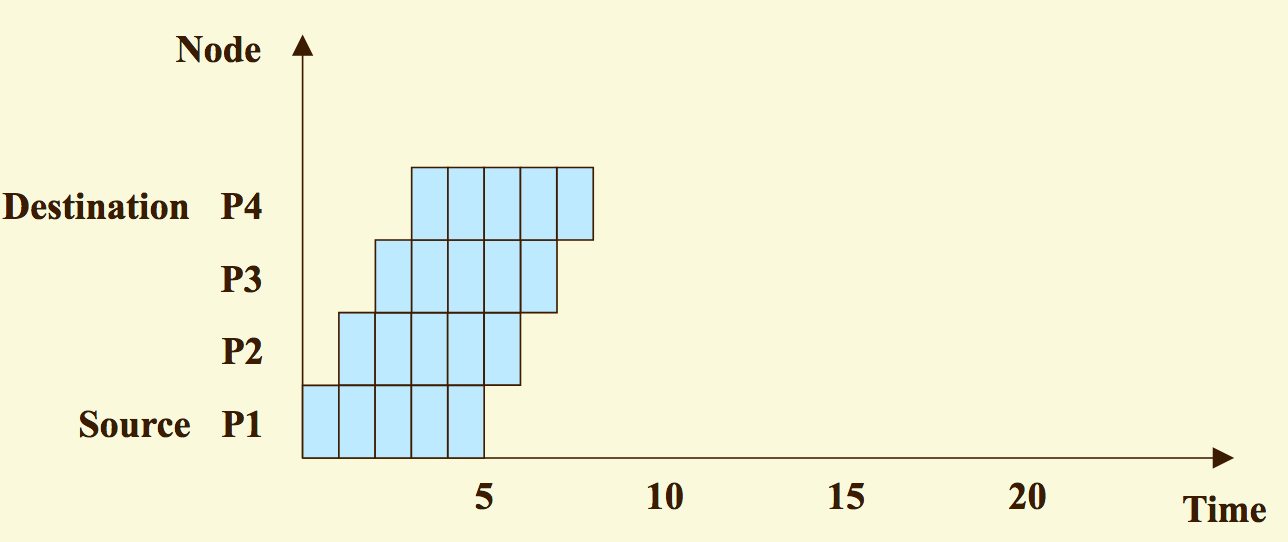
\includegraphics[width=0.7\linewidth]{screenshot133}
\caption{Network latency in virtual cut-through/wormhole routing.}
\label{fig:screenshot133}
\end{figure}


As long as the required channels are free, the message will be forwarded between the nodes FLIT-by-FLIT. If the channel is busy, FLITS are buffered at intermediate nodes. If the buffers are large enough, the entire message is buffered and the system will behave like packet switching. If the buffers are not large enough, the message will be buffered across several nodes holding the links.

Wormhole routing is a special-case of virtual cut-through where the buffer size is the size of a flit; it is depicted in \autoref{fig:screenshot130}. It is capable of packet replication, which is used to implement broadcasts - packets can be sent out on multiple output channels concurrently, which is not possible with circuit switching.

\begin{figure}
\centering
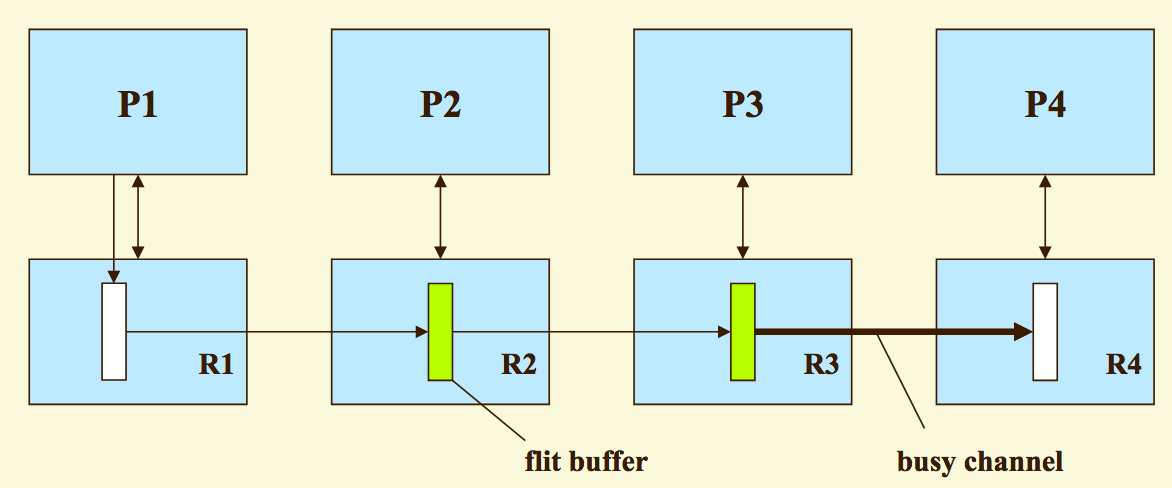
\includegraphics[width=0.7\linewidth]{screenshot130}
\caption{Wormhole routing.}
\label{fig:screenshot130}
\end{figure}

Wormhole routing is better than circuit switching when switch contention is high, as circuit switching blocks the path for the whole message. Wormhole routing breaks into FLITS, which leads to higher efficiency; however, if the path is blocked, the intermediate channels will also be blocked. Additionally, the contention may occur on intermediate nodes within the path.

\subsection{Virtual Channels}
Virtual channels allow multiple independent messages to share the same physical channels. This is done by \textit{multiplexing} multiple FLITS onto a single channel, such that the number of FLIT buffers exceeds that of the number of channels (depicted in \autoref{fig:screenshot134}).

\begin{figure}
\centering
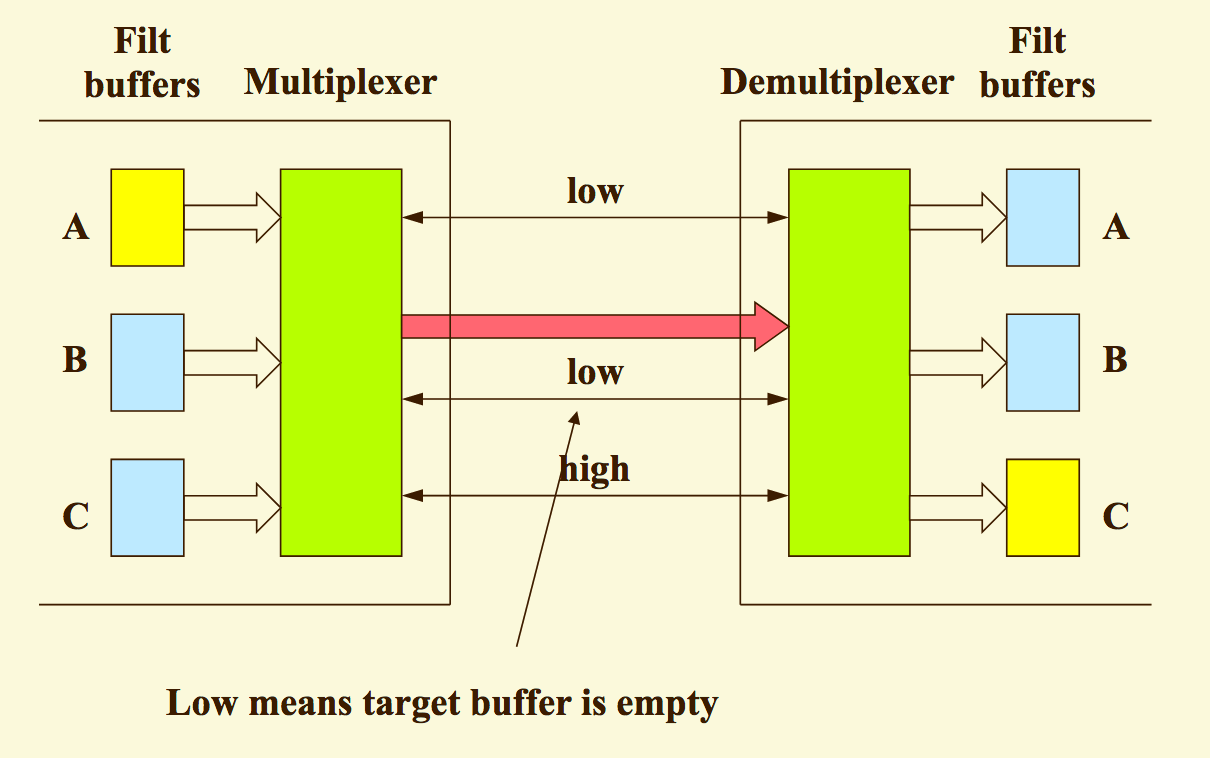
\includegraphics[width=0.7\linewidth]{screenshot134}
\caption{Virtual channels in routing.}
\label{fig:screenshot134}
\end{figure}

Virtual channels allow for increased network throughput by reducing the idle time of physical channels. They can also be used to avoid deadlocks. They allow the mapping of the logical topology of the network onto the physical network; as the mapping is not exact, some logical channels can be reserved for critical functions like debugging and monitoring.

A comparison between routing without virtual channels and routing with virtual channels is seen in \autoref{fig:screenshot135} and \autoref{fig:screenshot136} respectively.
\begin{figure}
\centering
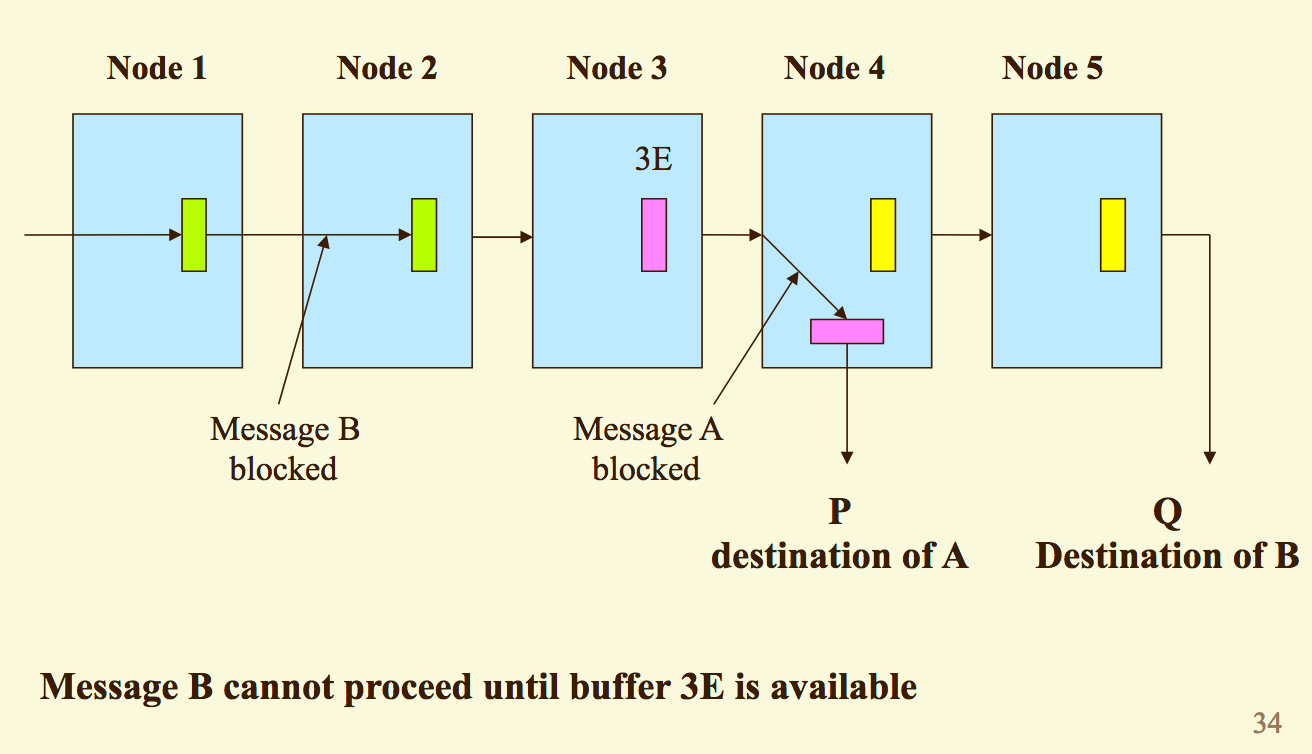
\includegraphics[width=0.7\linewidth]{screenshot135}
\caption{Routing without virtual channels.}
\label{fig:screenshot135}
\end{figure}

\begin{figure}
\centering
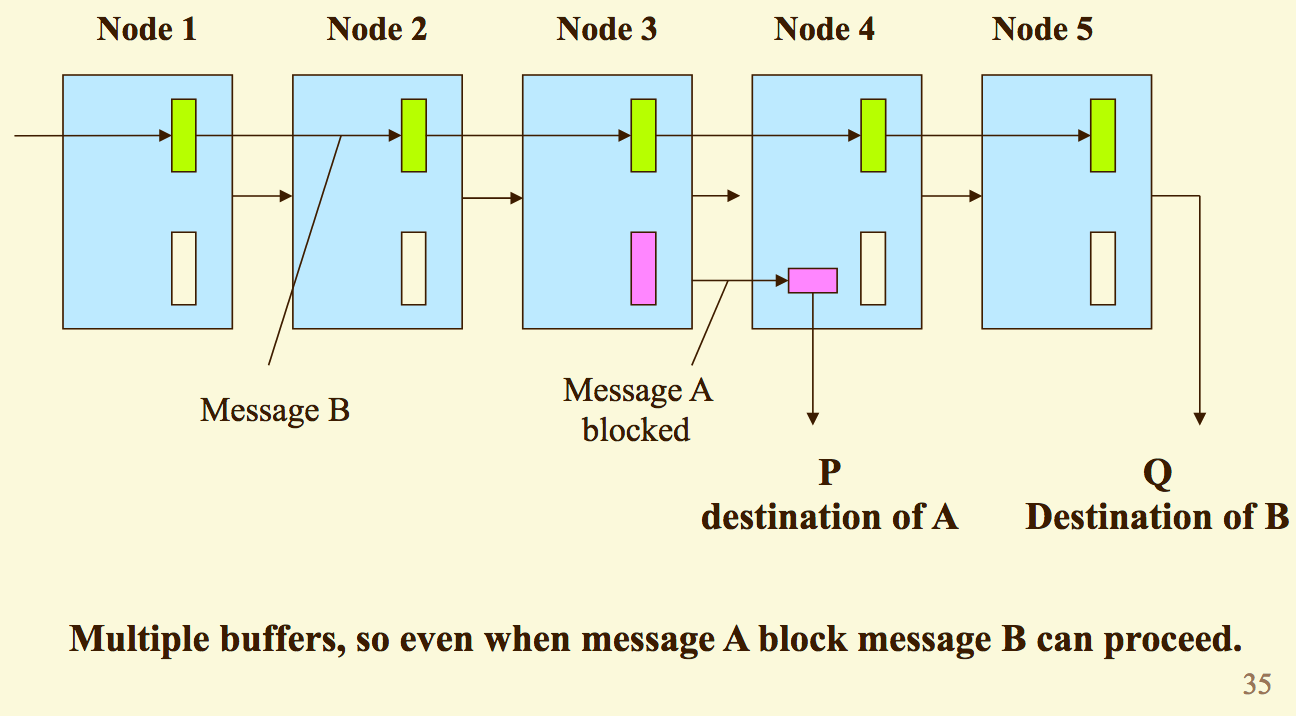
\includegraphics[width=0.7\linewidth]{screenshot136}
\caption{Routes with virtual channels.}
\label{fig:screenshot136}
\end{figure}

\subsection{Deadlocks}
Deadlocks can occur in scenarios like \autoref{fig:screenshot137}, where each node is waiting on a message from its neighbour. This is a \textit{cyclic dependency graph}, constructed from the interconnection network and routing algorithm. If cycles are present, deadlock may occur.

\begin{figure}
\centering
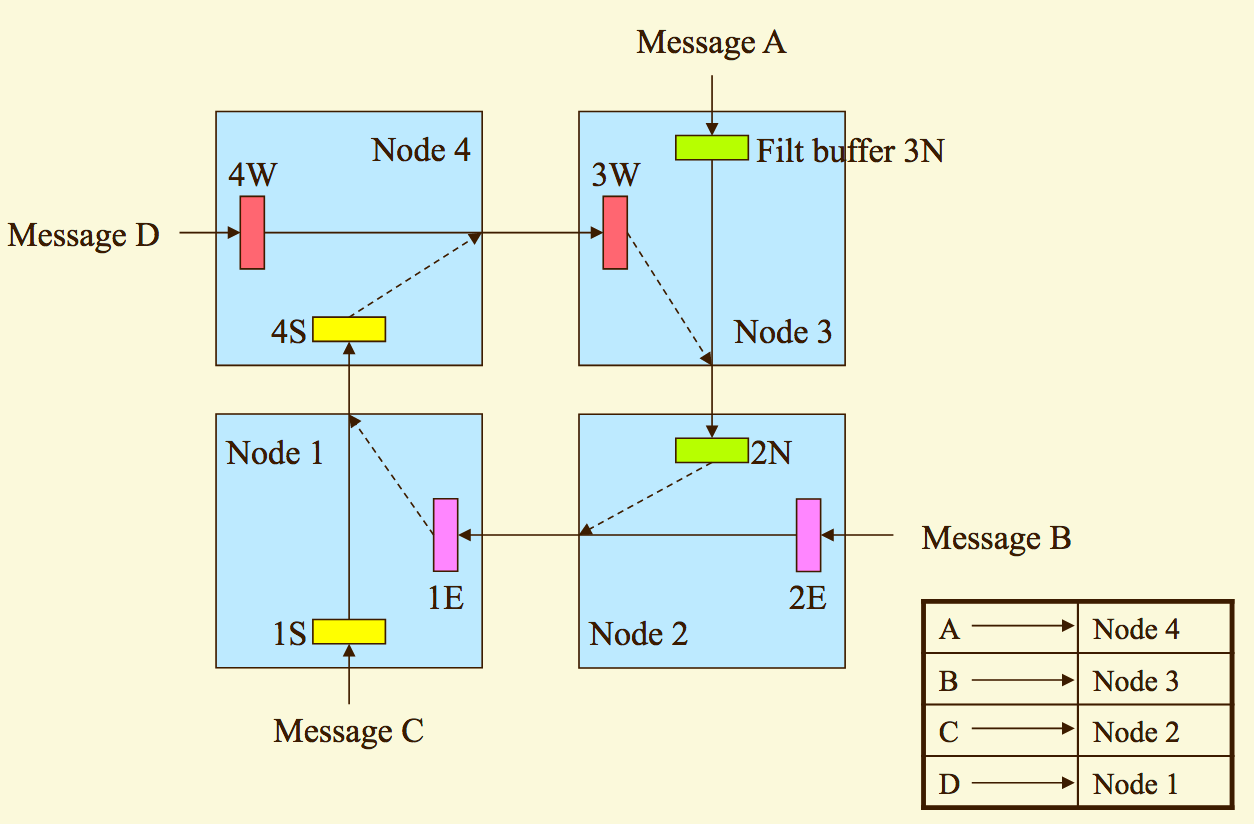
\includegraphics[width=0.7\linewidth]{screenshot137}
\caption{Typical deadlock scenario.}
\label{fig:screenshot137}
\end{figure}

Deadlocks can be avoided by: \begin{itemize}
\item pre-empting messages via rerouting (that is, using an alternate path for one message so that the cycle is broken)
\item pre-empting messages by discarding them and transmitting them on an alternate path
\item application of virtual channels; splitting physical channels into multiple virtual channels is sufficient to break cycles in the dependency graph
\end{itemize}

\subsection{Livelocks}
When a livelock occurs, a message is endlessly propagated through the network but fails to ever reach its destination. This can occur in flow control policies that avoid collisions on channels and buffers by misrouting messages to find an alternative path. Packet switching and virtual cut-through are very sensitive to livelock, but circuit switching and wormhole routing are typically livelock free.

\section{Routing protocols}
Routing protocols can be put in a hierarchy, as depicted in \autoref{fig:screenshot138}.

\begin{figure}
\centering
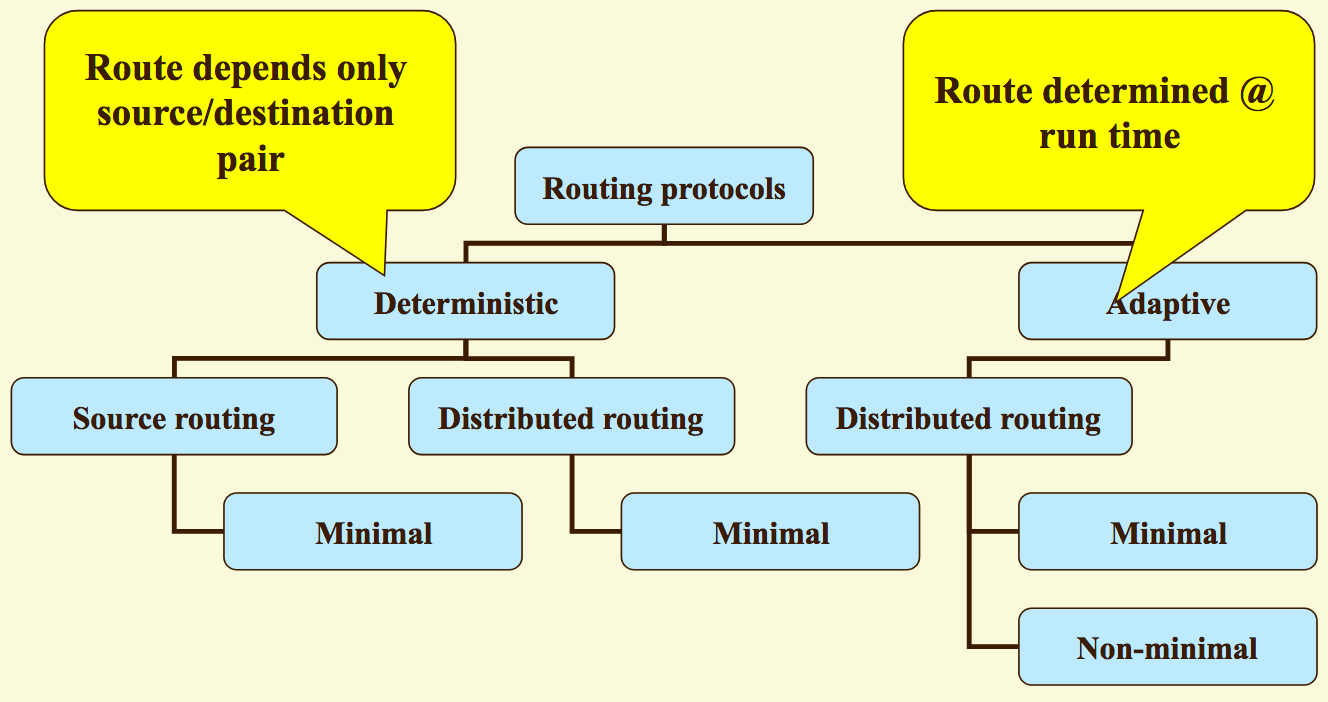
\includegraphics[width=0.7\linewidth]{screenshot138}
\caption{Routing protocol hierarchy.}
\label{fig:screenshot138}
\end{figure}

\subsection{Deterministic Routing}
In deterministic routing, the route depends only on the source and destination pair and no other information.

\subsubsection{Street Sign Routing}
In street sign routing, the message header contains the complete path information; the routing information is stored in the form of direction changes. This is shown in \autoref{fig:screenshot139}.

\begin{figure}
\centering
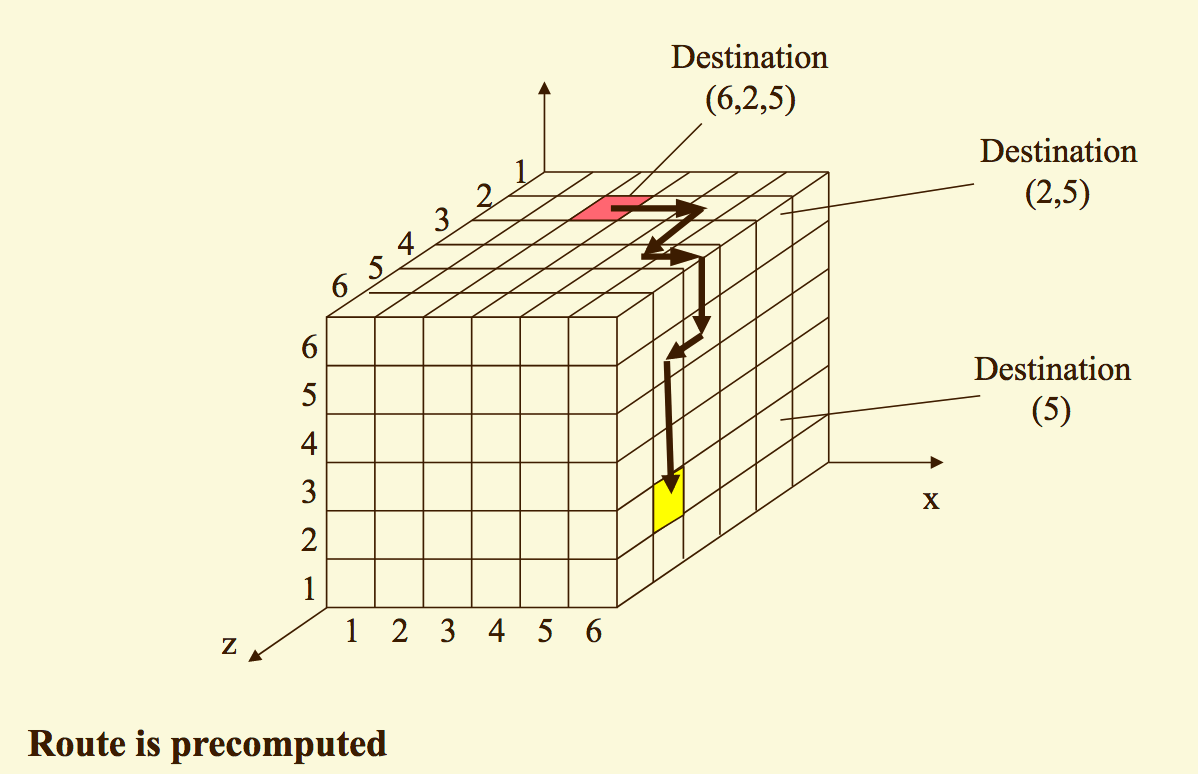
\includegraphics[width=0.7\linewidth]{screenshot139}
\caption{Street sign routing.}
\label{fig:screenshot139}
\end{figure}

\subsubsection{Dimension-ordered routing}
In dimension-ordered routing, the message travels along a certain dimension until it is aligned with the destination on that dimension. It will then proceed to do the same for each dimension until it reaches the destination. This is shown in \autoref{fig:screenshot140}.

\begin{figure}
\centering
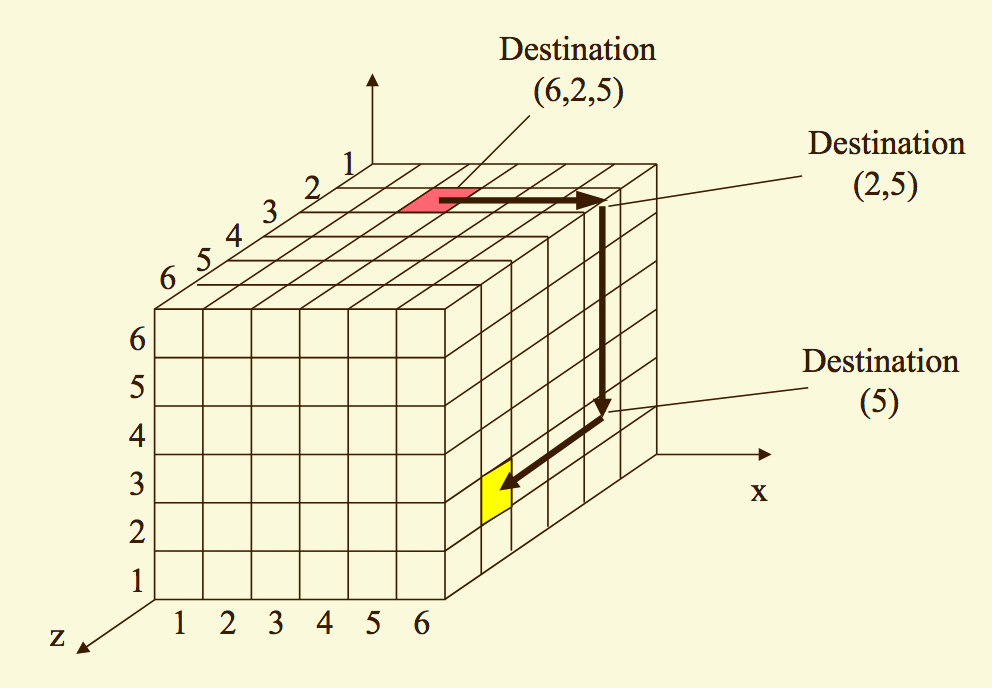
\includegraphics[width=0.7\linewidth]{screenshot140}
\caption{Dimension-ordered routing.}
\label{fig:screenshot140}
\end{figure}

\subsubsection{Table lookup routing}
In table lookup routing, each node contains a routing table. This table contains the identifier of the neighbouring node to which the message should be routed; there is one entry per destination address. The tables are precomputed and can be large.

\subsection{Adaptive Routing}
Adaptive routing protocols can be put in a hierarchy, as depicted in \autoref{fig:screenshot141}.

\begin{figure}
\centering
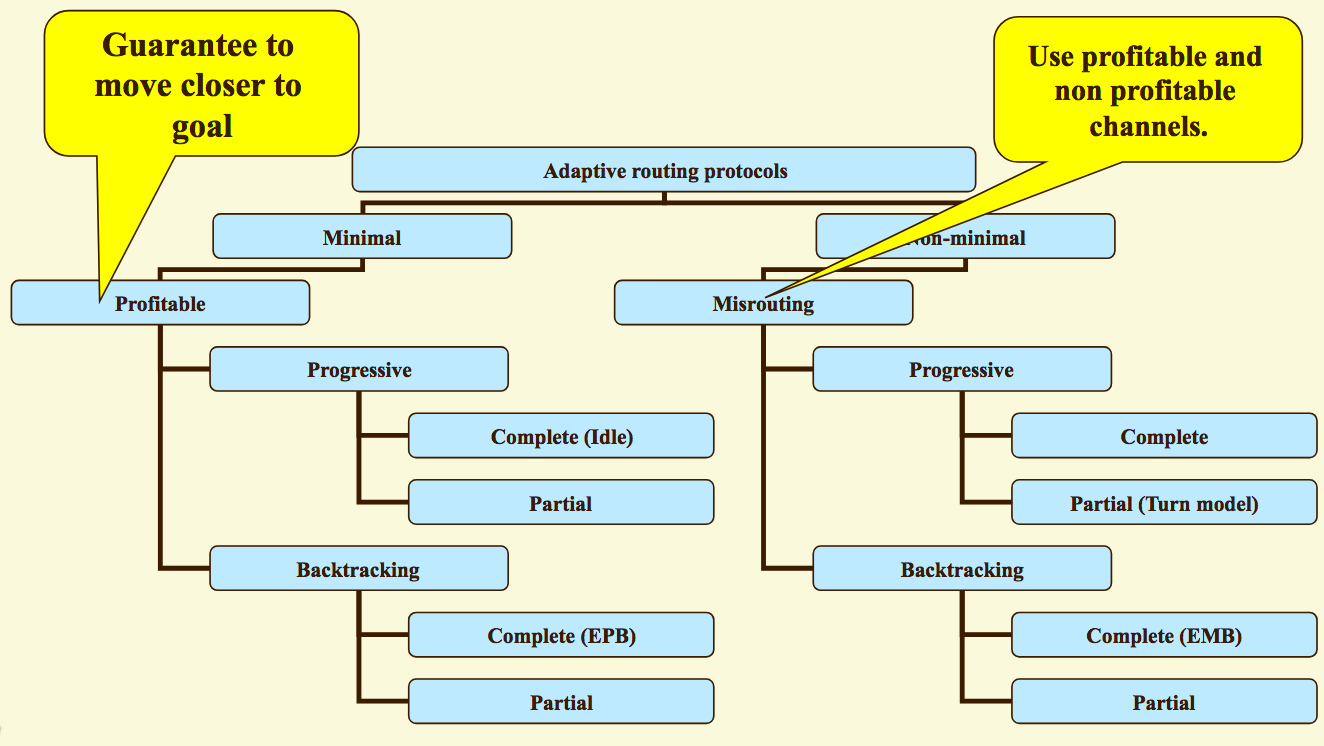
\includegraphics[width=0.7\linewidth]{screenshot141}
\caption{Adaptive routing protocols.}
\label{fig:screenshot141}
\end{figure}

\subsubsection{Profitable vs Misrouting}
Profitable protocols can only move closer to the goal and represent a conservative view. They will produce the minimum length path, are free from livelock, and are easier to prove deadlock free.

Misrouting protocols can take other choices and represent an optimistic view. They select a non-profitable channel in belief that it will lead to profitable ones. They are more fault tolerant as they do not have to use particular channels for their transmission.

\subsubsection{Progressive vs Backtracking}
Progressive protocols cannot backtrack, and may deadlock.

Backtracking protocols can systematically explore all paths and are deadlock free, but are more complex. They need to know where they have been before. If there are no profitable channels available (depending on whether the protocol is profitable or misrouting), the protocol will need to wait for a channel, try a non-profitable free channel, and if that fails step back and try again.

\subsubsection{Complete vs Partial}
A complete routing protocol can explore all channels, while a partial protocol can only use selected channels. A partial choice of channels allows a deadlock-free route to be computed. 

\begin{quote}
Add nodes used the same ordering of channels and explore them in this order.

e.g. West first: Route west as first choice then choose other directions adaptively 
\end{quote}

\section{Machine design choices}
MIMD systems can be built from processors that support any of the following: \begin{itemize}
\item Fine-grain message passing: J-Machine
\item Medium-grain message passing: Transputer (built around communicating sequential processes, or CSP)
\item Coarse-grain message passing: COTS; networks have higher latency, and the processors don't need to understand message passing
\end{itemize}

\subsection{Fine-grain}
Fine-grain concurrent processing reduces overhead and latency of receiving a message through hardware support. Hardware support additionally reduces context-switching time (through the use of multiple registers and hardware support for synchronisation). Object-oriented programming, when implemented in hardware, provides \texttt{call} and \texttt{send} operations to objects. The architecture of the J-Machine processor is shown in \autoref{fig:screenshot142}.

\begin{figure}
\centering
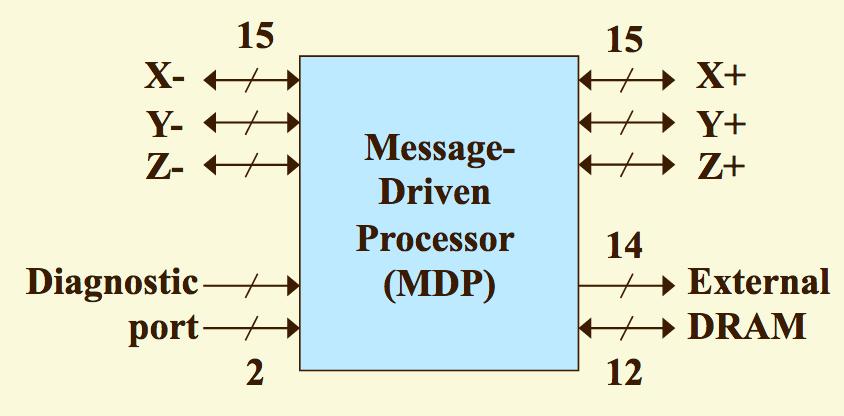
\includegraphics[width=0.7\linewidth]{screenshot142}
\caption{J-Machine processor architecture.}
\label{fig:screenshot142}
\end{figure}

\subsection{Medium-grain}
Message passing is synchronous; neither the sender or receiver can continue without each other. The first process reaching a channel operation must be suspended until the partner arrives. Transputer is an example of a medium-grain computer; it is depicted in \autoref{fig:screenshot143}.

\begin{figure}
\centering
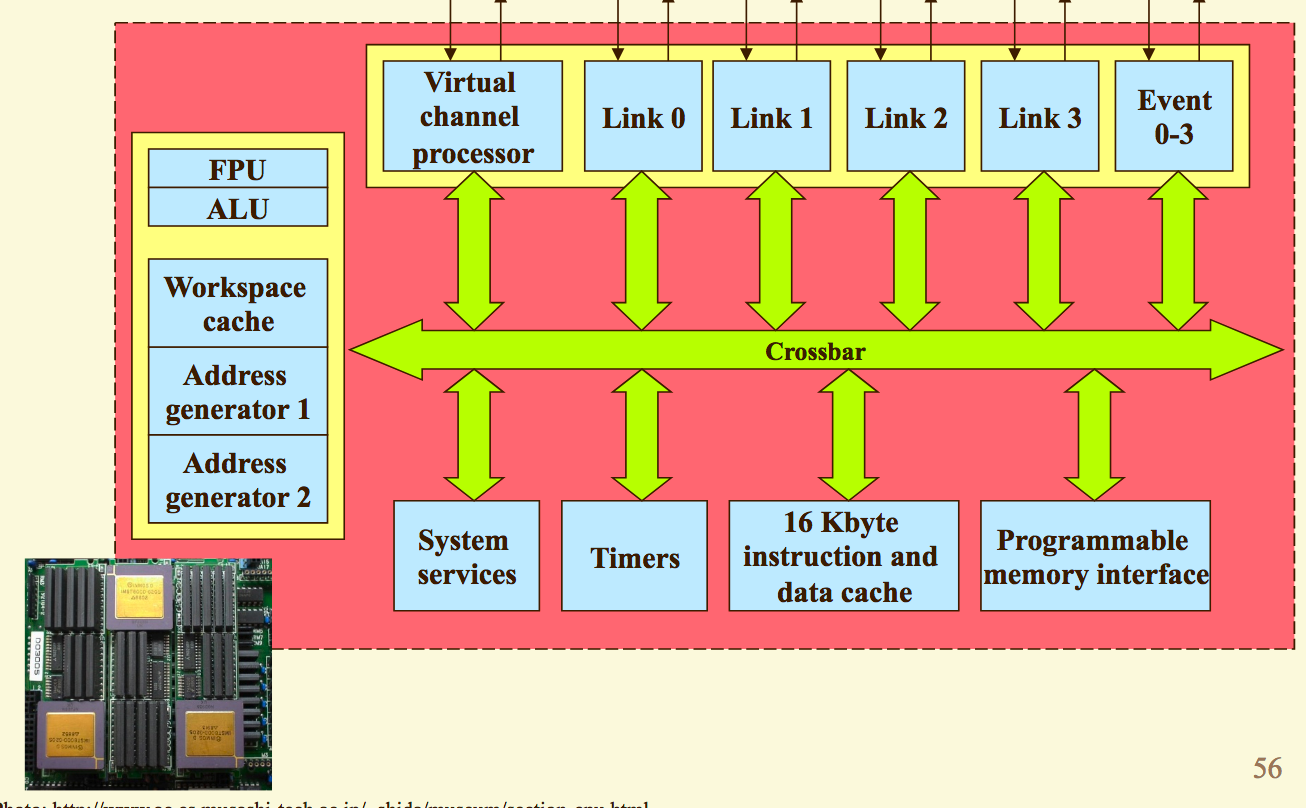
\includegraphics[width=0.7\linewidth]{screenshot143}
\caption{Medium-grain Transputer architecture.}
\label{fig:screenshot143}
\end{figure}

Running processes need to be statically mapped onto hardware; this includes links and processors. All processors are mapped onto a single Transputer; there are no external links used. This leads to an allocation diagram similar to the one in \autoref{fig:screenshot144}.

\begin{figure}
\centering
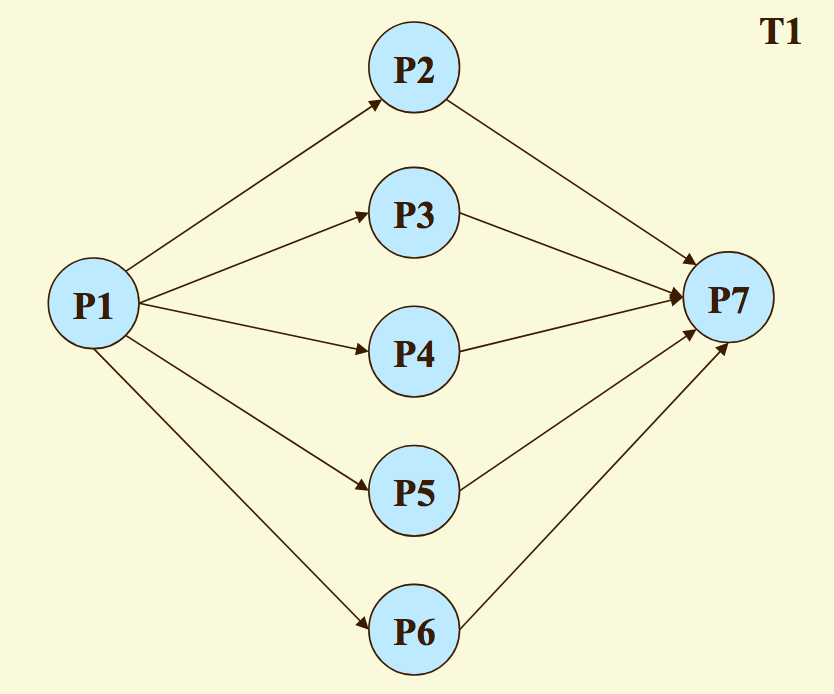
\includegraphics[width=0.7\linewidth]{screenshot144}
\caption{A single Transputer process allocation diagram.}
\label{fig:screenshot144}
\end{figure}

However, if more than one Transputer is used, it may not be possible to provide enough physical links to connect between all of them (as depicted in \autoref{fig:screenshot145}); this is solved using virtual links.

\begin{figure}
\centering
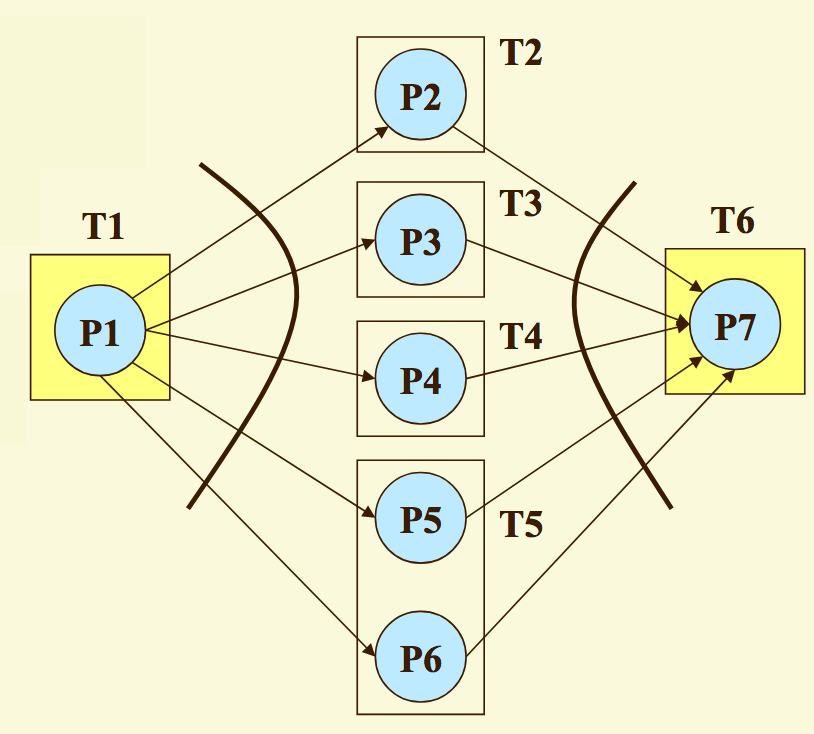
\includegraphics[width=0.7\linewidth]{screenshot145}
\caption{Too many physical links for a multi-Transputer arrangement.}
\label{fig:screenshot145}
\end{figure}

Transputers are traditionally connected using links to form a mesh; this mesh is routed using a C104 router chip, which provides a 32-way crossbar. This is depicted in \autoref{fig:screenshot146}.

\begin{figure}
\centering
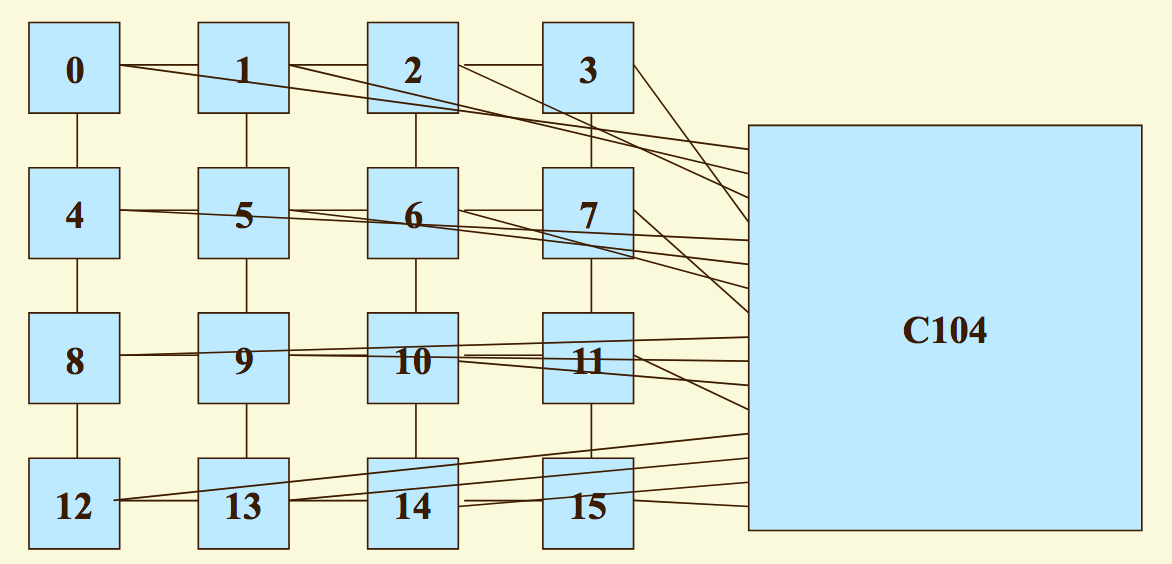
\includegraphics[width=0.7\linewidth]{screenshot146}
\caption{Transputer mesh.}
\label{fig:screenshot146}
\end{figure}

\subsection{Coarse-grain}
Finally, the design space for coarse-grain third-generation multicomputers is reproduced in \autoref{fig:screenshot147}.

\begin{figure}
\centering
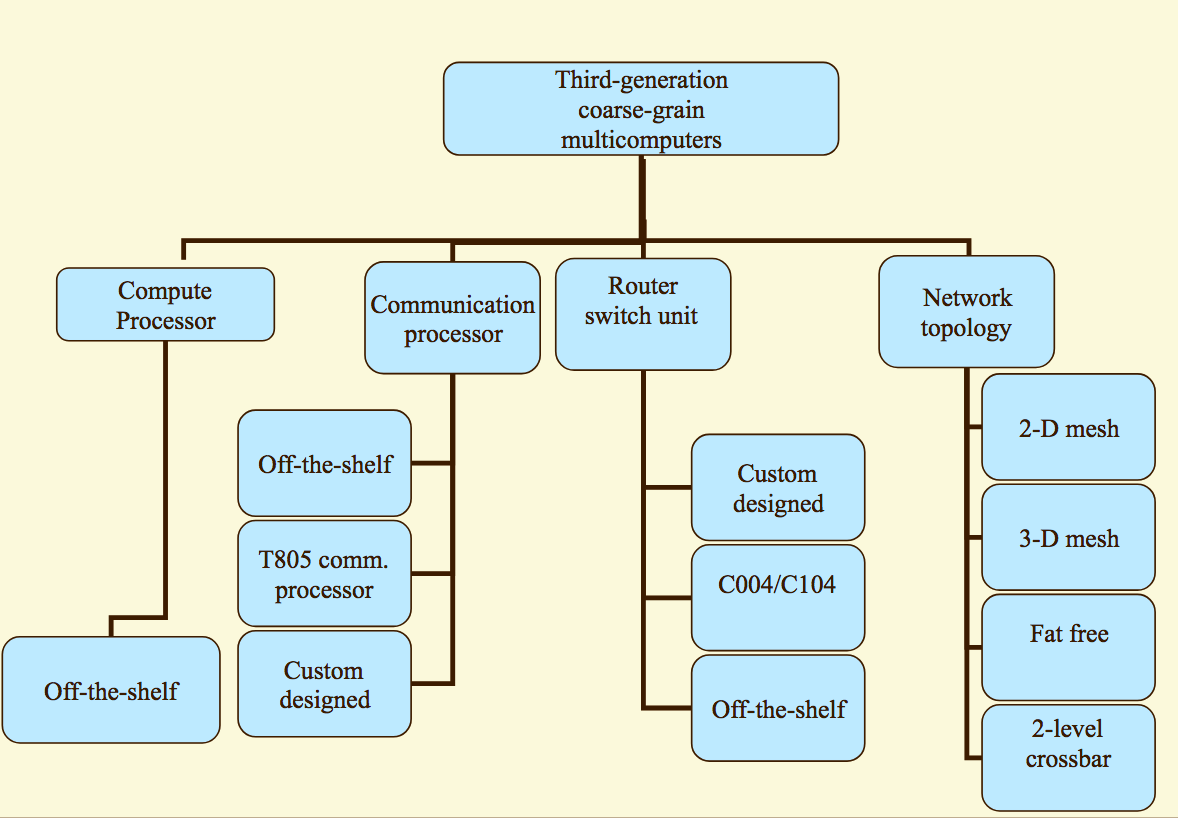
\includegraphics[width=\linewidth]{screenshot147}
\caption{Design-space of third-generation coarse-grain multicomputers.}
\label{fig:screenshot147}
\end{figure}
